\bta{验证机械能守恒定律}
\begin{enumerate}
\renewcommand{\labelenumi}{\arabic{enumi}.}
% A(\Alph) a(\alph) I(\Roman) i(\roman) 1(\arabic)
%设定全局标号series=example	%引用全局变量resume=example
%[topsep=-0.3em,parsep=-0.3em,itemsep=-0.3em,partopsep=-0.3em]
%可使用leftmargin调整列表环境左边的空白长度 [leftmargin=0em]
\item
$ 2016 $ 年上海卷 $ 26 $.($ 3 $ 分)在“用 $ DIS $ 研究机械能守恒定律”的实验中,用到的传感器是
\tk{光电门} 
传感器。若摆锤直径的测量值大于其真实值会造成摆锤动能的测量值偏
\tk{大} 
。
(选填:“大”或“小”)。







\item
\exwhere{$ 2017 $ 年天津卷}
如图所示,打点计时器固定在铁架台上,使重物带动纸带从静止开始自由
下落,利用此装置验证机械能守恒定律。

①对于该实验,下列操作中对减小实验误差有利的是 \tk{AB} 。
\begin{figure}[h!]
\centering
\includesvg[width=0.23\linewidth]{picture/svg/GZ-3-tiyou-0466}
\end{figure}


\fourchoices
{重物选用质量和密度较大的金属锤}
{两限位孔在同一竖直面内上下对正}
{精确测量出重物的质量}
{用手托稳重物,接通电源后,撒手释放重物}


②某实验小组利用上述装置将打点计时器接到 $ 50 \ Hz $ 的交流电源上,按
正确操作得到了一条完整的纸带,由于纸带较长,图中有部分未画出,如图所示。纸带上各点是打
点计时器打出的计时点,其中 $ O $ 点为纸带上打出的第一个点。重物下落高度应从纸带上计时点间的
距离直接测出,利用下列测量值能完成验证机械能守恒定律的选项有 \tk{BC} 。
\begin{figure}[h!]
\centering
\includesvg[width=0.43\linewidth]{picture/svg/GZ-3-tiyou-0467}
\end{figure}

\fourchoices
{$ OA $、$ AD $ 和 $ EG $ 的长度}
{$ OC $、$ BC $ 和 $ CD $ 的长度}
{$ BD $、$ CF $ 和 $ EG $ 的长度}
{$ AC $、$ BD $ 和 $ EG $ 的长度}





\newpage

\item
\exwhere{$ 2013 $ 年海南卷}
某同学用图($ a $)所示的实验装置验证机械能守恒定律。已知打点计时器所用电源的频率为 $ 50 \ Hz $,
当地重力加速度为 $ g=9.80 \ m/s^{2} $。实验中该同学
得到的一条点迹清晰的完整纸带如图($ b $)所示。
纸带上的第一个点记为 $ O $,另选连续的三个点
$ A $、$ B $、$ C $ 进行测量,图中给出了这三个点到 $ O $
点的距离 $ h_{A} $、$ h_{B} $ 和 $ h_{C} $ 的值。回答下列问题(计
算结果保留 $ 3 $ 位有效数字)
\begin{figure}[h!]
\centering
\includesvg[width=0.53\linewidth]{picture/svg/GZ-3-tiyou-0469}
\end{figure}


\begin{enumerate}
\renewcommand{\labelenumi}{\arabic{enumi}.}
% A(\Alph) a(\alph) I(\Roman) i(\roman) 1(\arabic)
%设定全局标号series=example	%引用全局变量resume=example
%[topsep=-0.3em,parsep=-0.3em,itemsep=-0.3em,partopsep=-0.3em]
%可使用leftmargin调整列表环境左边的空白长度 [leftmargin=0em]
\item
打点计时器打 $ B $ 点时,重物速度的大小 $ v_{B} = $
\tk{$ 3.90 $} 
$ m/s $;

\item 
通过分析该同学测量的实验数据,他的实验结果是否验证了机械能守恒定律?简要说明分析
的依据。

\tk{$ 3.90 $($ 2 $)$ v_{B} ^{2}/2=7.61(m/s)^{2} $,因为 $ m v_{B} ^{2}/2 \approx mg h_{B} $,近似验证机械能守恒定律} 

\end{enumerate}




\newpage
\item
\exwhere{$ 2015 $ 年理综浙江卷}
甲同学准备做“验证机械能守恒定律”实验,乙同学准备做“探究加
速度与力、质量的关系”实验。
% TODO: \usepackage{graphicx} required
\begin{figure}[h!]
\centering
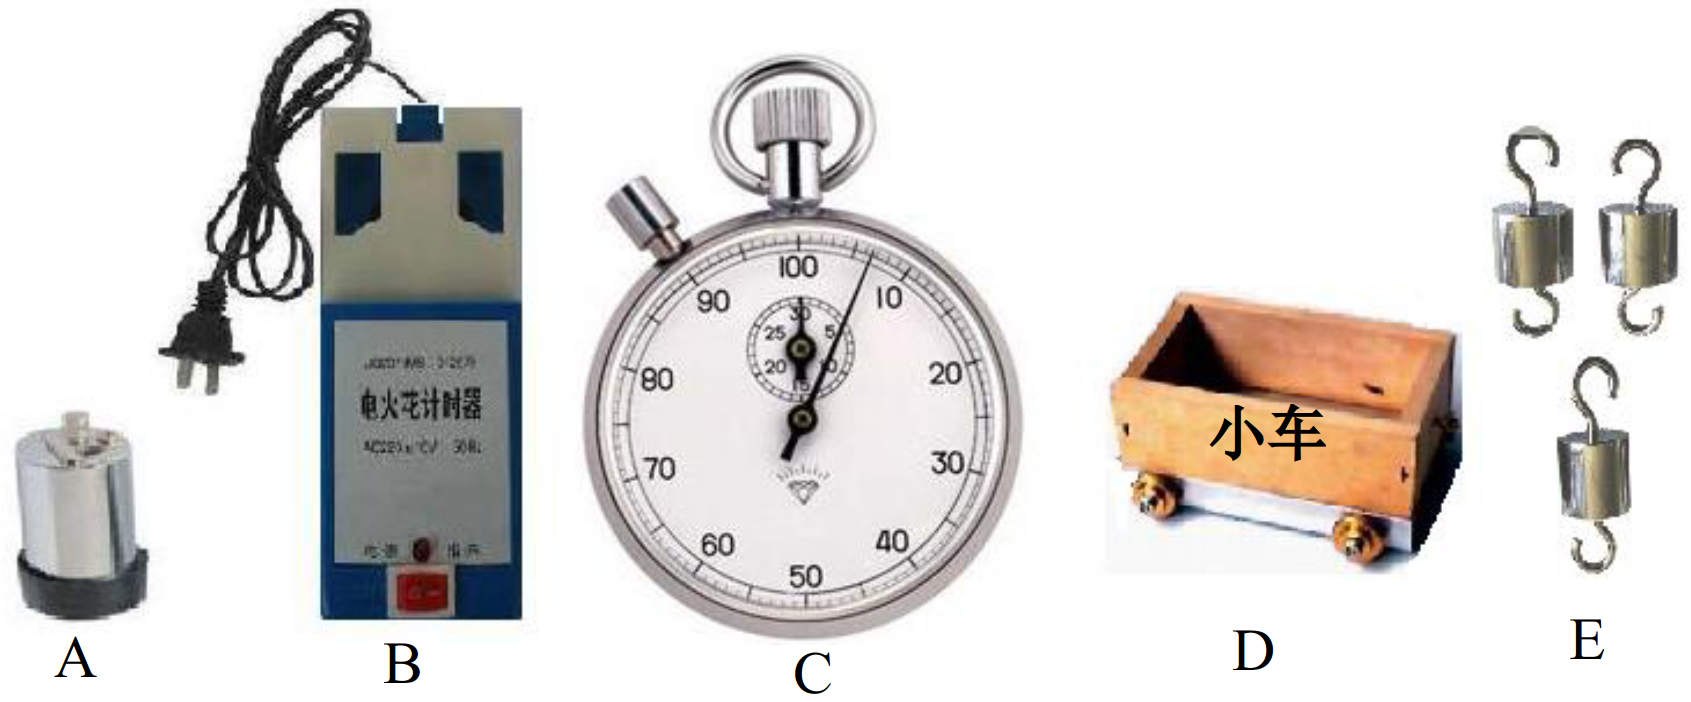
\includegraphics[width=0.7\linewidth]{picture/screenshot032}
\end{figure}

\begin{enumerate}
\renewcommand{\labelenumi}{\arabic{enumi}.}
% A(\Alph) a(\alph) I(\Roman) i(\roman) 1(\arabic)
%设定全局标号series=example	%引用全局变量resume=example
%[topsep=-0.3em,parsep=-0.3em,itemsep=-0.3em,partopsep=-0.3em]
%可使用leftmargin调整列表环境左边的空白长度 [leftmargin=0em]
\item
图 $ 1 $ 中 $ A $、$ B $、$ C $、$ D $、$ E $
表示部分实验器材,甲同学需
在图中选用的器材 \tk{AB} ;
乙同学需在图中选用的器材
\tk{BDE} 。(用字母表示)


\item 
乙同学在实验室选齐所
需器材后,经正确操作获得如
图 $ 2 $ 所示的两条纸带①和②。纸带 \tk{①} 的加速度大(填①或者②)
,其加速度大小为 \tk{$ (2.5 \pm 0.2) \ m/s^{2} $} 
。
\begin{figure}[h!]
\centering
\includesvg[width=0.73\linewidth]{picture/svg/GZ-3-tiyou-0470}
\end{figure}



\end{enumerate}


\newpage
\item 
\exwhere{$ 2011 $ 年海南卷}
现要通过实验验证机械能守恒定律。实验装置如图 $ 1 $ 所示:水平桌面上固定一倾斜的气垫导轨;
导轨上 $ A $ 点处有一带长方形遮光片的滑块,其总质量为 $ M $,左端由跨过轻质光滑定滑轮的细绳与一
质量为 $ m $ 的砝码相连;遮光片两条长边与导轨垂直;导轨上 $ B $ 点有一光电门,可以测量遮光片经
过光电门时的挡光时间 $ t $。用 $ d $ 表示 $ A $ 点到导轨低端 $ C $ 点的距离,$ h $ 表示 $ A $ 与 $ C $ 的高度差,$ b $ 表示
遮光片的宽度,$ s $ 表示 $ A $,$ B $ 两点的距离,将遮光片通过光电门的平均速度看作滑块通过 $ B $ 点时的
瞬时速度。用 $ g $ 表示重力加速度。完成下列填空和作图;
\begin{figure}[h!]
\centering
\includesvg[width=0.3\linewidth]{picture/svg/GZ-3-tiyou-0471}
\end{figure}

\begin{enumerate}
\renewcommand{\labelenumi}{\arabic{enumi}.}
% A(\Alph) a(\alph) I(\Roman) i(\roman) 1(\arabic)
%设定全局标号series=example	%引用全局变量resume=example
%[topsep=-0.3em,parsep=-0.3em,itemsep=-0.3em,partopsep=-0.3em]
%可使用leftmargin调整列表环境左边的空白长度 [leftmargin=0em]
\item
若将滑块自 $ A $ 点由静止释放,则在滑块从 $ A $ 运动至 $ B $ 的
过程中,滑块、遮光片与砝码组成的系统重力势能的减小量可
表示为
\tk{$\left(\frac{h}{d} M-m\right) g s$} 
。动能的增加量可表示为
\tk{$\frac{1}{2}(M+m) \frac{b^{2}}{t^{2}}$} 
。若在运
动过程中机械能守恒,
$ \frac{1}{t^{2}} $
与 $ s $ 的关系式为 $\frac{1}{t^{2}}=$ \tk{$\frac{2(h M-d m) g}{(M+m) d b^{2}} s$} 。





\item 
多次改变光电门的位置,每次均令滑块自同一点($ A $ 点)下滑,测量相应的 $ s $ 与 $ t $ 值,结果如下
表所示:

\begin{table}[h!]
\centering 
\begin{tabular}{|c|c|c|c|c|c|}
\hline 
& $ 1 $ & $ 2 $ & $ 3 $ & $ 4 $ & $ 5 $
 \\
\hline
$ s(m) $ & $ 0.600 $ & $ 0.800 $ & $ 1.000 $ & $ 1.200 $ & $ 1.400 $
 \\
\hline
$ t(ms $) & $ 8.22 $ & $ 7.17 $ & $ 6.44 $ & $ 5.85 $ & $ 5.43 $
 \\
\hline
$ 1/ t^{2} (10^4 \ s^{-2}) $ & $ 1.48 $ & $ 1.95 $ & $ 2.41 $ & $ 2.92 $ & $ 3.39 $\\ 
\hline 
\end{tabular}
\end{table} 




以 $ s $ 为横坐标,
$\frac{1}{t^{2}}$
为纵坐标,在答题卡上对应图 $ 2 $ 位置的坐标纸中描出第 $ 1 $ 和第 $ 5 $ 个数据点;根
据 $ 5 $ 个数据点作直线,求得该直线的斜率 $ k= $
\tk{40} 
$ \times 10^{4} \ m^{-1} \cdot s^{-2} $(保留 $ 3 $ 位有效数字)。
\vspace{-3em}
\begin{figure}[h!]
\centering
\includesvg[width=0.43\linewidth]{picture/svg/GZ-3-tiyou-0472}
\end{figure}

\banswer{
 \includesvg[width=0.23\linewidth]{picture/svg/GZ-3-tiyou-0473} 
}


由测得的 $ h $、$ d $、$ b $、$ M $ 和 $ m $ 数值可以计算出
$\frac{1}{t^{2}}-s$直线的斜率 $ k_{0} $,将 $ k $ 和 $ k_{0} $ 进行比较,若其差值在
试验允许的范围内,则可认为此试验验证了机械
能守恒定律。

\end{enumerate}




\newpage
\item
\exwhere{$ 2016 $ 年新课标 \lmd{1} 卷}
某同学用图($ a $)所示的实验装置验证机械能守恒定律,其中打点计
时器的电源为交流电源,可以使用的频率有 $ 20 \ Hz $、$ 30 \ Hz $ 和 $ 40 \ Hz $。
打出纸带的一部分如图($ b $)所示。
\begin{figure}[h!]
\centering
\includesvg[width=0.23\linewidth]{picture/svg/GZ-3-tiyou-0474} \qquad \includesvg[width=0.53\linewidth]{picture/svg/GZ-3-tiyou-0475} 
\end{figure}


该同学在实验中没有记录交流电的频率 $ f $,需要用实验数据和其它题
给条件进行推算。

\begin{enumerate}
\renewcommand{\labelenumi}{\arabic{enumi}.}
% A(\Alph) a(\alph) I(\Roman) i(\roman) 1(\arabic)
%设定全局标号series=example	%引用全局变量resume=example
%[topsep=-0.3em,parsep=-0.3em,itemsep=-0.3em,partopsep=-0.3em]
%可使用leftmargin调整列表环境左边的空白长度 [leftmargin=0em]
\item
若从打出的纸带可判定重物匀加速下落,利用 $ f $ 和图($ b $)中给出
的物理量可以写出:在打点计时器打出 $ B $ 点时,重物下落的速度大小
为 \tk{$\frac{f}{2}\left(S_{1}+S_{2}\right)$} ,打出 $ C $ 点时重物下落的速度大小为 \tk{$\frac{f}{2}\left(S_{2}+S_{3}\right)$} 
,重物下落的加速度大小为 \tk{$\frac{f^{2}}{2}\left(S_{3}-S_{1}\right)$} 
。



\item 
已测得 $ S_1=8.89 \ cm $,$ S_2=9.50 \ cm $,$ S_3=10.10 \ cm $, 当地重力加速度大小为 $ 9.80 \ m/s^{2} $,实验中重
物受到的平均阻力大小约为其重力的 $ 1 \% $,由此推算出 $ f $ 为 \tk{$ 40 $} $ Hz $。


\end{enumerate}



\newpage
\item 
\exwhere{$ 2016 $ 年北京卷}
\begin{enumerate}
\renewcommand{\labelenumi}{\arabic{enumi}.}
% A(\Alph) a(\alph) I(\Roman) i(\roman) 1(\arabic)
%设定全局标号series=example	%引用全局变量resume=example
%[topsep=-0.3em,parsep=-0.3em,itemsep=-0.3em,partopsep=-0.3em]
%可使用leftmargin调整列表环境左边的空白长度 [leftmargin=0em]
\item
热敏电阻常用于温度控制或过热保护装置中。图 $ 1 $ 为某种热敏电阻和金属热电阻的阻值 $ R $ 随
温度 $ t $ 变化的示意图。由图可知,这种热敏电阻在温度上升时导电能力
\tk{增强} 
(选填“增强”或“减弱”)
;相对金属热电阻而言,热敏电阻
对温度变化的影响更
\tk{敏感} 
(选填“敏感”或“不敏感”)
。
\begin{figure}[h!]
\centering
\includesvg[width=0.23\linewidth]{picture/svg/GZ-3-tiyou-0476} \qquad 
 \includesvg[width=0.14\linewidth]{picture/svg/GZ-3-tiyou-0477} 
\end{figure}


\item 
利用图 $ 2 $ 装置做“验证机械能守恒定律”实验。

①为验证机械能是否守恒,需要比较重物下落过程中任意两点间
的 \tk{A} 。
\threechoices
{动能变化量与势能变化量}
{速度变化量和势能变化量}
{速度变化量和高度变化量}

②除带夹子的重物、纸带、铁架台(含铁夹)
、电磁打点计时器、导线及开关外,在下列器材中,
还必须使用的两种器材是 \tk{AB} 。
\threechoices
{交流电源}
{刻度尺}
{天平(含砝码)}

③实验中,先接通电源,再释放重物,得到图 $ 3 $ 所示的一条纸带。在纸带上选取三个连续打出的点
$ A $、$ B $、$ C $,测得它们到起始点 $ O $ 的距离分别为
$ h_{A} $、$ h_{B} $、$ h_{C} $。
\begin{figure}[h!]
\centering
\includesvg[width=0.48\linewidth]{picture/svg/GZ-3-tiyou-0478}
\end{figure}


已知当地重力加速度为 $ g $,打点计时器打点的周
期为 $ T $。设重物的质量为 $ m $。从打O点到打B点
的过程中,重物的重力势能变化量$ \Delta E_{p} = $
\tk{$ -mg h_{B} $} 
,动能变化量$ \Delta E_{k} = $
\tk{$\frac{1}{2} m\left(\frac{h_{\mathrm{C}}-h_{\mathrm{A}}}{2 T}\right)^{2}$}。

④大多数学生的实验结果显示,重力势能的减少量大于动能的增加量,原因是 \tk{C} 
\fourchoices
{利用公式 $ v=gt $ 计算中午速度}
{利用公式 $ v=2 \ g h $计算重物速度}
{存在空气阻力和摩擦力阻力的影响}
{没有采用多次试验去平均值的方法}

\item
某同学想用下述方法研究机械能是否守恒,在纸带上选取多个计数点,测量它们到起始点 $ O $ 的
○
距离 $ h $,计算对应计数点的重物速度 $ v $,描绘 $ v_{2} -h $ 图像,并做如下判断:若图像是一条过原点的直
线,则重物下落过程中机械能守恒,请你分析论证该同学的判断是否正确。


\tk{⑤该同学的判断依据不正确} 

\end{enumerate}



\newpage
\item 
\exwhere{$ 2016 $ 年江苏卷}
某同学用如图 $ 1 $ 所示的装置验证机械能守恒定律。一根细线系住钢球,悬
挂在铁架台上,钢球静止于 $ A $ 点,光电门固定在 $ A $ 的正下方。
在钢球底部竖直地粘住一片宽度为 $ d $ 的遮光条.将钢球拉至
不同位置由静止释放,遮光条经过光电门的挡光时间 $ t $ 可由
计时器测出,取 $v=\frac{d}{t}$
作为钢球经过 $ A $ 点时的速度.记录钢
球每次下落的高度 $ h $ 和计时器示数 $ t $,计算并比较钢球在释放
点和 $ A $ 点之间的势能变化大小$ \Delta E_{p} $ 与动能变化大小$ \Delta E_{k} $,就能
验证机械能是否守恒。
\begin{figure}[h!]
\centering
\includesvg[width=0.3\linewidth]{picture/svg/GZ-3-tiyou-0479}
\end{figure}

\begin{enumerate}
\renewcommand{\labelenumi}{\arabic{enumi}.}
% A(\Alph) a(\alph) I(\Roman) i(\roman) 1(\arabic)
%设定全局标号series=example	%引用全局变量resume=example
%[topsep=-0.3em,parsep=-0.3em,itemsep=-0.3em,partopsep=-0.3em]
%可使用leftmargin调整列表环境左边的空白长度 [leftmargin=0em]
\item
用$ \Delta E_{p} =mgh $ 计算钢球重力势能变化的大小,式中钢球下落
高度 $ h $ 应测量释放时的钢球球心到 \tk{B} 之间的竖直距离。
\threechoices
{钢球在 $ A $ 点时的顶端}
{钢球在 $ A $ 点时的球心}
{钢球在 $ A $ 点时的底端}



\item 
用$ \Delta E_{k} = \frac{ 1 }{ 2 } m v_{2} $ 计算钢球动能变化的大小,用刻度尺测量遮光条宽度,示数如图 $ 2 $ 所示,其读数
为 \tk{$ 1.50(1.49 \sim 1.51 $ 都算对)} $ cm $。某次测量中,计时器的示数为 $ 0.0100 \ s $,则钢球的速度为 $ v=$ \tk{$ 1.50(1.49 \sim 1.51 $ 都算对)} $m/s $。
\begin{figure}[h!]
\centering
\includesvg[width=0.23\linewidth]{picture/svg/GZ-3-tiyou-0480}
\end{figure}



\item 
下表为该同学的实验结果:
\begin{table}[h!]
\centering 
\begin{tabular}{|c|c|c|c|c|c|}
\hline 
$ \Delta E_{p} /(10^{-2} \ J) $ & $ 4.892 $ & $ 9.786 $ & $ 14.69 $ & $ 19.59 $ & $ 29.38 $
 \\
\hline
$ \Delta E_{k} /(10^{-2} \ J) $ & $ 5.04 $ & $ 10.1 $ & $ 15.1 $ & $ 20.0 $ & $ 29.8 $\\ 
\hline 
\end{tabular}
\end{table} 


他发现表中的$ \Delta E_{p} $ 与$ \Delta E_{k} $ 之间存在差异,认为这是由于空气阻力造成的。你是否同意他的观点?请
说明理由。

\tk{不同意,因为空气阻力会造成$ \Delta E_{k} $ 小于$ \Delta E_{p} $,但表中$ \Delta E_{k} $ 大于$ \Delta E_{p} $。} 

\item 
请你提出一条减小上述差异的改进建议。

\tk{分别测出光电门和球心到悬点的长度 $ L $ 和 $ l $,计算$ \Delta E_{k} $ 时,将 $ v $ 折算成钢球的速度 $ v ^{\prime} =\frac{l}{L}v $。} 

\end{enumerate}







\end{enumerate}

